\chapter{Data Conversion Service Specification}
\section*{\textit{Version 1.0}}
\section{Introduction}

A conscious design decision was made for CIShell not to enforce a central data
model/format that all algorithms had to work with. Instead, an algorithm
expresses in its service metadata for each data item coming into and out of the
algorithm what the format of the data is. It is the job of the code calling the
algorithm to get the data in the right format before calling the algorithm. The
Data Conversion Service is used here to simplify the process of converting data.

\subsection{Entities}

\begin{itemize}
  \item \textit{DataConversionService} - The service interface for converting
  data to different formats.
  \item \textit{Converter Algorithm} - A special type of algorithm, defined
  on page \pageref{converterAlg}, which converts data from one format to
  another.
  \item \textit{Converter} - The interface for a wrapped set of converter
  algorithms returned by the \class{DataConversionService} that will convert
  data from one format to another.
\end{itemize}

\section{Data Conversion Service}

The Data Conversion Service provides unified access to converter algorithms.
\class{DataConversionService} system developers may choose not to leverage
converter algorithms, but this is ill-advised. Also, good implementations will
take advantage of the nature of converter algorithms to allow for more than just
single hop conversions. Since all converter algorithms specify a single data
object in and a single data object out, a graph can be constructed where nodes
are the data formats and edges are the converters. Using this directed graph,
when a conversion between data formats is requested, the
\class{DataConversionService} will choose the shortest path of converters to do
the conversion. A hypothetical conversion graph is illustrated in figure
\ref{fig:conversionGraph}.

\begin{figure}[h!]
\centering
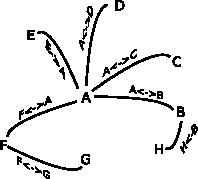
\includegraphics[width=70mm]{../img/conversionGraph.pdf}
\caption{A Conversion Graph}
\label{fig:conversionGraph}
\end{figure}

\orgcishellserviceconversion{}